\documentclass{article}
\usepackage{geometry} % Required for customizing margins
\geometry{margin=1in} % Sets 1-inch margins on all sides
\usepackage{listings}
\usepackage{amsmath}
\usepackage{tikz}
\usepackage{titlesec}  % For customizing section/subsection titles
\usetikzlibrary{arrows}

% Custom format for sections and subsections
\titleformat{\section}[block]{\normalfont\Large\bfseries}{\thesection}{1em}{}
\titleformat{\subsection}[block]{\normalfont\large\bfseries}{\thesubsection}{1em}{}

% Page layout settings
\geometry{
    top=1.0in,
    bottom=1.0in,
    left=1.0in,
    right=1.0in
}

\begin{document}

% Horizontal line
\hrule
\vspace{0.2cm}

% Centered title
\begin{center}
    \LARGE \textbf{CSCE 350} \\
    \Large Data Structures and Algorithms \\
    \large HW \#2
\end{center}

% Horizontal line
\hrule
\vspace{0.2cm}

% Author and semester info
\begin{center}
    \textbf{Author:} Jacob Vaught \\
    \vspace{0.2cm}
    \textbf{Semester:} Fall 2023 \\
\end{center}

% Another horizontal line
\hrule
\vspace{0.5cm}

\newpage
\section*{Problem \#1[Figure 1]}
\begin{center}
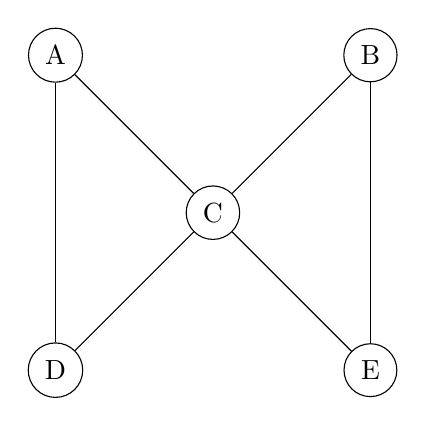
\begin{tikzpicture}[scale=2]
  \node[shape=circle,draw=black] (A) at (0,2) {A};
  \node[shape=circle,draw=black] (B) at (2,2) {B};
  \node[shape=circle,draw=black] (C) at (1,1) {C};
  \node[shape=circle,draw=black] (D) at (0,0) {D};
  \node[shape=circle,draw=black] (E) at (2,0) {E};
  \path [-] (A) edge node {} (C);
  \path [-] (B) edge node {} (C);
  \path [-] (D) edge node {} (C);
  \path [-] (E) edge node {} (C);
  \path [-] (A) edge node {} (D);
  \path [-] (B) edge node {} (E);
\end{tikzpicture}
\end{center}

\begin{enumerate}
    \item Write down the adjacency matrix and adjacency list for the graph.
    \item Determine if there are any cycles in the graph. If so, write down the corresponding paths.
\end{enumerate}

\subsection*{Solution}

\subsubsection*{Adjacency Matrix[7 Points]}

For the given graph, the adjacency matrix would look like:

\[
\begin{pmatrix}
0 & 0 & 1 & 1 & 0 \\
0 & 0 & 1 & 0 & 1 \\
1 & 1 & 0 & 1 & 1 \\
1 & 0 & 1 & 0 & 0 \\
0 & 1 & 1 & 0 & 0 \\
\end{pmatrix}
\]

\subsubsection*{Adjacency List[7 Points]}

The adjacency list for the graph would be:

\begin{itemize}
    \item \(A: [C, D]\)
    \item \(B: [C, E]\)
    \item \(C: [A, B, D, E]\)
    \item \(D: [A, C]\)
    \item \(E: [B, C]\)
\end{itemize}

\subsubsection*{Cycles in the Graph[2.5 Points]}

Upon inspecting the graph, we can see that there are cycles present. Specifically:

\begin{itemize}
    \item \(A \rightarrow C \rightarrow D \rightarrow A\)
    \item \(B \rightarrow C \rightarrow E \rightarrow B\)
    \item \(C \rightarrow A \rightarrow D \rightarrow C\)
    \item \(C \rightarrow B \rightarrow E \rightarrow C\)
\end{itemize}

\newpage
\section*{Problem \#1[Figure 2]}
\begin{center}
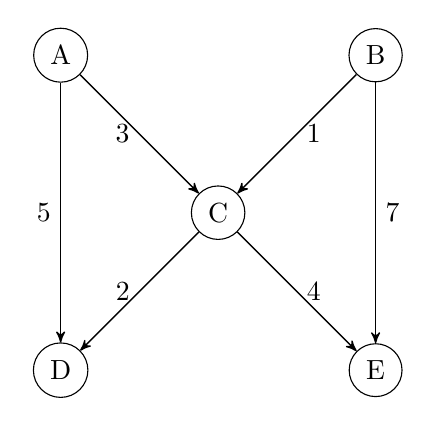
\begin{tikzpicture}[scale=2, > = latex'] % The 'latex'' option sets the arrowhead style
  \node[shape=circle,draw=black] (A) at (0,2) {A};
  \node[shape=circle,draw=black] (B) at (2,2) {B};
  \node[shape=circle,draw=black] (C) at (1,1) {C};
  \node[shape=circle,draw=black] (D) at (0,0) {D};
  \node[shape=circle,draw=black] (E) at (2,0) {E};
  
  \path [->, line width=0.5pt, >=stealth', scale=2] (A) edge node[midway, left] {3} (C);
  \path [->, line width=0.5pt, >=stealth', scale=2] (A) edge node[midway, left] {5} (D);
  \path [->, line width=0.5pt, >=stealth', scale=2] (B) edge node[midway, right] {1} (C);
  \path [->, line width=0.5pt, >=stealth', scale=2] (B) edge node[midway, right] {7} (E);
  \path [->, line width=0.5pt, >=stealth', scale=2] (C) edge node[midway, left] {2} (D);
  \path [->, line width=0.5pt, >=stealth', scale=2] (C) edge node[midway, right] {4} (E);
\end{tikzpicture}
\end{center}

\begin{enumerate}
    \item Write down the adjacency matrix and adjacency list for the graph.
    \item Determine if there are any cycles in the graph. If so, write down the corresponding paths.
\end{enumerate}

\subsection*{Solution}

\subsubsection*{Adjacency Matrix[7 Points]}

For the given directed graph, the adjacency matrix would look like:

\[
\begin{pmatrix}
0 & 0 & 3 & 5 & 0 \\
0 & 0 & 1 & 0 & 7 \\
0 & 0 & 0 & 2 & 4 \\
0 & 0 & 0 & 0 & 0 \\
0 & 0 & 0 & 0 & 0 \\
\end{pmatrix}
\]

\subsubsection*{Adjacency List[7 Points]}

The adjacency list for the graph would be:

\begin{itemize}
    \item \(A: [(C, 3), (D, 5)]\)
    \item \(B: [(C, 1), (E, 7)]\)
    \item \(C: [(D, 2), (E, 4)]\)
    \item \(D: [ - ]\)
    \item \(E: [ - ]\)
\end{itemize}

\subsubsection*{Cycles in the Graph[2.5 Points]}

Upon inspecting the graph, we can see that there are no cycles present. All paths are directed, and there is no way to start and end at the same node while following the edge directions.

\newpage
\section*{Problem \#2}
For each of the following functions, indicate the class \( \Theta(g(n)) \) the function belongs to. Use the simplest \( g(n) \) possible in your answers. Prove your assertions using limits. Show your work.

\begin{itemize}
    \item \([7 \text{ points}]\) \( (n^2+n)^{10} \)
    \item \([10 \text{ points}]\) \( n \log[n^2]+(n-2)^2 \log \left( \frac{n}{2} \right) \)
\end{itemize}

\subsection*{Solutions}
\subsubsection*{(a.) \( (n^2+n)^{10} \)[15 Points]}
The function \( f(n) = (n^2+n)^{10} \) belongs to \( \Theta(n^{20}) \).
\newline
\textit{Proof:}
\[
\lim_{{n \to \infty}} \frac{(n^2+n)^{10}}{n^{20}} = \lim_{{n \to \infty}} \left( 1+\frac{1}{n} \right)^{10} = 1
\]
\newline
Since the limit is a constant value that is not zero or infinity, we can conclude \( f(n) = \Theta(n^{20}) \).
\newline
\newline
\subsubsection*{(b.) \( n \log[n^2]+(n-2)^2 \log \left( \frac{n}{2} \right) \)[15 Points]}

The function \( f(n) = n \log[n^2]+(n-2)^2 \log \left( \frac{n}{2} \right) \) belongs to \( \Theta(n^2) \).
\newline 
\newline
\textit{Proof:}
\newline 
First term:
\[
\lim_{{n \to \infty}} \frac{n \log[n^2]}{n^2} = \lim_{{n \to \infty}} \frac{2 \log n}{n} = 0
\]
This indicates that \( n \log[n^2] = o(n^2) \).
Second term:
\[
\lim_{{n \to \infty}} \frac{(n-2)^2 \log \left( \frac{n}{2} \right)}{n^2} = \lim_{{n \to \infty}} \frac{(n-2)^2 \log n - (n-2)^2 \log 2}{n^2} = 1 - \lim_{{n \to \infty}} \frac{4(n-2)}{n^2} = 1
\]
Since the limit is a constant that is not zero or infinity, we can conclude \( (n-2)^2 \log \left( \frac{n}{2} \right) = \Theta(n^2log(n)) \).


\newpage
\section*{Problem \#3}
Solve the following sums. The final answer must be listed in terms of ‘n’. Show your work. 
\newline
Find their orders of growth using the simplest g(n) possible.


\subsection*{a. \( \sum_{{i=0}}^{{n-1}} (i^2 - 2)^2 \)}

To find the sum, we first expand the term \( (i^2 - 2)^2 \):
\[
(i^2 - 2)^2 = i^4 - 4i^2 + 4
\]
Now, summing these terms from \( i=0 \) to \( i=n-1 \) gives:
\[
\begin{aligned}
\sum_{{i=0}}^{{n-1}} (i^4 - 4i^2 + 4) &= \sum_{{i=0}}^{{n-1}} i^4 - 4\sum_{{i=0}}^{{n-1}} i^2 + 4\sum_{{i=0}}^{{n-1}} 1 \\
&= \frac{(n-1)(2n-1)(n)(3n^2 - 3n - 1)}{30} - 4\frac{(n-1)(2n-1)(n)}{6} + 4n \\
&= \frac{n(n-1)(2n-1)(3n^2 - 3n - 1)}{30} - \frac{2n(n-1)(2n-1)}{5} + 4n
\end{aligned}
\]
The dominant term here is \( n^5 \), so \( \Theta(n^5) \).

\subsection*{b. \( \sum_{{i=0}}^{{n-1}} \sum_{{j=0}}^{{i-1}} (i+j) \)}

The inner sum can be written as:
\[
\begin{aligned}
\sum_{{j=0}}^{{i-1}} (i+j) &= i(i-1) + \frac{(i-1)i}{2} \\
&= \frac{2i^2 - i}{2} + \frac{i(i-1)}{2} \\
&= i^2 - \frac{i}{2} \\
&= \frac{2i^2 - i}{2}
\end{aligned}
\]
Now we sum this term from \( i=0 \) to \( i=n-1 \):
\[
\begin{aligned}
\sum_{{i=0}}^{{n-1}} \frac{2i^2 - i}{2} &= \frac{1}{2} \left( 2\sum_{{i=0}}^{{n-1}} i^2 - \sum_{{i=0}}^{{n-1}} i \right) \\
&= \frac{1}{2} \left( 2\frac{(n-1)(2n-1)(n)}{6} - \frac{(n-1)n}{2} \right) \\
&= \frac{n(n-1)(n-2)}{6}
\end{aligned}
\]
The dominant term here is \( n^3 \), so \( \Theta(n^3) \).

\newpage
\section*{Problem \#4}
\subsection*{Consider the following algorithm}

\begin{verbatim}
ALGORITHM Unpack(n)
// Input: A non-negative integer n
S ← 0
for i ← 1 to n do
    S ← S + i * i * i
return S
\end{verbatim}

\subsubsection*{a. What does this algorithm compute?}

This algorithm computes the sum of the cubes of all integers from \(1\) to \(n\). Mathematically, it calculates:

\[
S = 1^3 + 2^3 + 3^3 + \ldots + n^3 = \sum_{{i=1}}^{n} i^3
\]

\subsubsection*{b. What is its basic operation?}

The basic operation of this algorithm is the cube and sum operation within the for-loop:

\[
S \leftarrow S + i \times i \times i
\]
\newline
This line is responsible for calculating the cube of \(i\) and adding it to the running sum \(S\).

\subsubsection*{c. How many times is the basic operation executed?}

The basic operation is executed \(n\) times. The for-loop iterates from \(1\) to \(n\), and during each iteration, the basic operation is performed exactly once.

\subsubsection*{d. What is the efficiency class of this algorithm?}

The algorithm's efficiency class is determined by the number of times the basic operation is executed, which is \(n\) times. Since the number of basic operations is linearly dependent on \(n\), the efficiency class of this algorithm is \( \Theta(n) \).
\newline \newline
In summary, this algorithm has linear time complexity, which makes it relatively efficient for calculating the sum of cubes for a given non-negative integer \( n \).

\end{document}